\begin{frame}
%\frametitle{There is more than just classification}
\frametitle{To explain or to predict?}
\begin{center}
{\huge ``\emph{The only relevant test of the validity of a hypothesis is comparison of prediction with experience}.''\par}
\vspace{1cm}
Milton Friedman
\end{center}
\end{frame}

\begin{frame}
\frametitle{To explain or to predict?}

\begin{quote}
``The predictive point of view is a prototypical point of view to explain the basic activity of statistical analysis.''
\par \rightline{\tiny{\rm --- Akaike}}
\end{quote}

\begin{quote}
``The only useful function of a statistician is to make predictions.''
\par \rightline{\tiny{\rm --- Deming}}
\end{quote}

\begin{quote}
``The prediction of observables or potential observables is of much greater relevance than the estimate of what are often artificial constructs-parameters''
\par\rightline{\tiny{\rm --- Geisser}}
\end{quote}
\vspace{.25cm}
\begin{center}
\begin{tiny}
Galit Shmueli. ``To Explain or to Predict?''. Statistical Science 25(3):289--310 (2010).
\end{tiny}
\end{center}
\end{frame}

%\begin{frame}
%\frametitle{To explain or to predict?}
%\begin{quote}
%%I should like to say a little about Heisenberg's idea that you should not talk about what you can not measure, because many people talk about this idea without really understanding it.
%You can interpret this in the sense that the {\bf construct or inventions that you make must be of such a kind that the consequences that you compute are comparable with experiment} - that is, that you do not compute a consequence like a `moo must be three goos', when nobody knows what a moo or a goo is.
%%  Obviously that is no good.  But if the consequences can be compared to experiment, then that is all that is necessary.  It does not matter that moos and goos cannot appear in the guess.  You can have as much junk in the guess as you like, provided that the consequences can be compared with experiment.  This is not always fully appreciated...\\
%...\\
%....{\bf Science is only useful if it tells you about some experiment that has not been done; it is no good if it only tells you what just went on.}
%\par \rightline{\tiny{\rm --- Richard Feynman; The Character of Physical Law}}
%\end{quote}
%\end{frame}


%\begin{frame}
%\frametitle{Choosing models/hypotheses/theories}
%\begin{columns}[c]
%\column{.3\textwidth}
%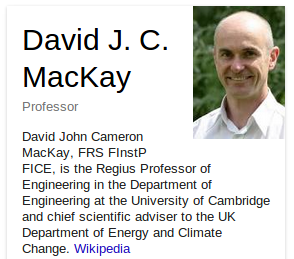
\includegraphics[width=\textwidth]{mackay}
%\vspace{.5cm}
%{\small
%MacKay, DJC. ``Bayesian interpolation.'' Neural computation 4, no. 3 (1992): 415-447.\par}
%\column{.7\textwidth}
%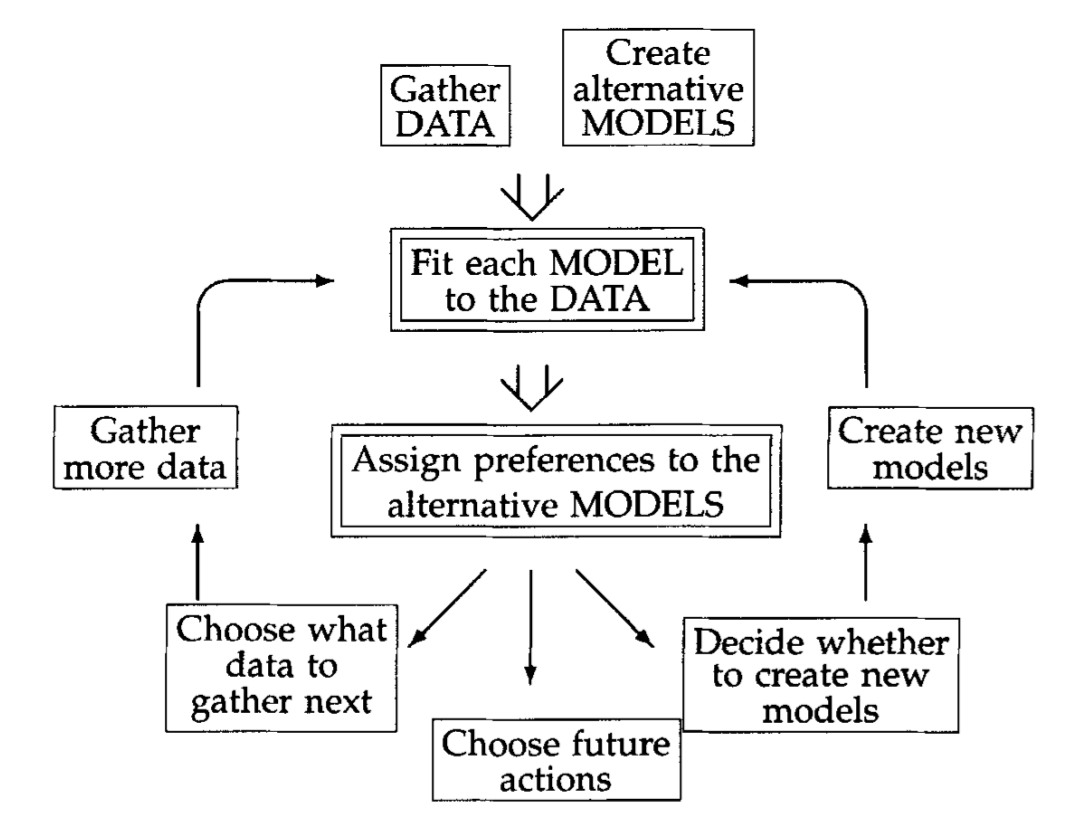
\includegraphics[width=\textwidth]{mackay1992}
%\end{columns}
%\end{frame}

\begin{frame}
\frametitle{Evidence-based Science}
...also just known as ``science''.
\vspace{0.5cm}
\begin{itemize}
\item{Researchers claim to find differences between groups.  Do those findings actually discriminate?}
\item{How can we most accurately diagnose a disorder from image data?}
\item{Pharma wants biomarkers.  How do we most effectively identify them?}
\item{There are lots of potential imaging biomarkers.  Which are most (cost) effective?}
\end{itemize}

Pattern recognition provides a framework to compare data (or preprocessing strategy) to determine the most accurate approach.
\end{frame}

\begin{frame}
\frametitle{Inter-subject Variability}
Why focus on anatomy?
\begin{itemize}
\item{Many medical applications involve understanding differences among individuals/populations.}
\item{In image data, most of the differences we can see are anatomical in nature.}
\item{Understanding growth and development requires us to look at growth and development (anatomy).}
\end{itemize}
\end{frame}

%\begin{frame}
%\frametitle{Cause and Effect}
%\begin{itemize}
%\item Anatomical data are generally purely observational (ie there's no intervention).
%\item Usually not possible to determine causality from such data.
%\item Causality is useful because it tells us something about outcomes from interventions.
%\item Usually in science, we predict dependent data (effects) from independent data (causes).
%\end{itemize}
%\end{frame}

\begin{frame}
\frametitle{Bayesian approaches may be better for clinical applications}
\begin{itemize}
\item Deals with different priors.
\begin{itemize}
\item Consider a method with 90\% sensitivity and specificity.
\item Consider using this to screen for a disease afflicting 1\% of the population.
\item On average, out of 100 people there would be 10 wrongly assigned to the disease group.
\item A positive diagnosis suggests only about a 10\% chance of having the disease.
{\small
\begin{eqnarray*}
P(\text{Disease} | \text{Pred+}) & = \frac{P(\text{Pred+} | \text{Disease}) P(\text{Disease})}{P(\text{Pred+} | \text{Disease}) P(\text{Disease}) + P(\text{Pred+} | \text{Healthy}) P(\text{Healthy})}\cr
% & = \frac{\text{Sensitivity} \times P(\text{Disease})}{\text{Sensitivity} \times P(\text{Disease}) + (1-Specificity) \times P(\text{Healthy})}
\end{eqnarray*}
\par
}
\end{itemize}
\item Better decision-making by accounting for utility functions.
\item Confidence may differ from subject to subject.
\end{itemize}
\end{frame}

%\begin{frame}
%\frametitle{Decision-making under uncertainty}
%\begin{itemize}
%\item Clinical decision-making is like gambling.
%\item Optimal way to gamble is Bayesian.
%\item ``Dutch Book Theorem''.
%\end{itemize}
%\end{frame}

